\documentclass[12pt,a4paper]{article}
\usepackage[a4paper, margin=0.8in, headheight=14pt]{geometry}
\usepackage{fontspec}
\usepackage{unicode-math}
\setmainfont{TeX Gyre Pagella}
\setmonofont[Scale=0.88]{TeX Gyre Cursor}
\setmathfont{Latin Modern Math}
\usepackage{xcolor}
\usepackage{colortbl}
\usepackage{titlesec}
\usepackage{enumitem}
\usepackage{tabularx}
\usepackage{booktabs}
\usepackage{array}
\usepackage{amsmath}
\usepackage{tikz}
\usetikzlibrary{shapes.geometric, arrows.meta, positioning, calc, fit, decorations.pathreplacing}
\usepackage{tcolorbox}
\tcbuselibrary{skins, breakable}
\usepackage{hyperref}
\usepackage{fancyhdr}
\usepackage{graphicx}
\usepackage{microtype}
\hyphenpenalty=10000
\exhyphenpenalty=10000
\sloppy
\usepackage{caption}
\usepackage{setspace}
\usepackage{multirow}
\usepackage{tocloft}
\newcommand{\Q}[1]{\textbf{#1}\par\noindent\ignorespaces}
\definecolor{myred}{RGB}{196,30,58}
\definecolor{mydark}{RGB}{30,30,50}
\definecolor{mygreen}{RGB}{14,120,80}
\definecolor{myteal}{RGB}{0,130,140}
\definecolor{myamber}{RGB}{180,100,0}
\definecolor{mypurple}{RGB}{100,30,160}
\definecolor{mygray}{RGB}{246,247,249}
\definecolor{mgframe}{RGB}{180,185,200}
\definecolor{watermark}{RGB}{145,150,170}
\definecolor{hdrred}{RGB}{250,232,235}
\definecolor{hdrgreen}{RGB}{220,244,233}
\definecolor{hdrteal}{RGB}{220,242,244}
\definecolor{hdramber}{RGB}{253,242,215}
\definecolor{hdrpurple}{RGB}{238,228,255}
\definecolor{hdrgray}{RGB}{238,240,245}
\definecolor{rowalt}{RGB}{250,251,253}
\titleformat{\section}{\large\bfseries\color{myred}}{\thesection.}{0.5em}{}[\vspace{1pt}{\color{myred}\rule{\linewidth}{0.8pt}}]
\titleformat{\subsection}{\normalsize\bfseries\color{myteal}}{\thesubsection}{0.5em}{}
\titlespacing*{\section}{0pt}{18pt}{7pt}
\titlespacing*{\subsection}{0pt}{11pt}{4pt}
\setlength{\parindent}{0pt}
\setlength{\parskip}{4pt}
\renewcommand{\cfttoctitlefont}{\large\bfseries\color{myred}}
\renewcommand{\cftaftertoctitle}{\par\noindent{\color{myred}\rule{\linewidth}{0.8pt}}}
\setlength{\cftbeforetoctitleskip}{0pt}
\setlength{\cftaftertoctitleskip}{6pt}
\renewcommand{\cftsecfont}{\normalsize\bfseries\color{mydark}}
\renewcommand{\cftsecpagefont}{\normalsize\bfseries\color{mydark}}
\renewcommand{\cftsecleader}{\cftdotfill{\cftdotsep}}
\setlength{\cftbeforesecskip}{7pt}
\renewcommand{\cftsubsecfont}{\small\color{mydark}}
\renewcommand{\cftsubsecpagefont}{\small\color{mydark}}
\setlength{\cftbeforesubsecskip}{3pt}
\setlength{\cftsubsecindent}{1.4em}
\renewcommand{\arraystretch}{1.45}
\setlength{\tabcolsep}{6pt}
\arrayrulecolor{mydark}
\newcolumntype{B}[1]{>{\small\bfseries\raggedright\arraybackslash}m{#1}}
\newcolumntype{Y}{>{\small\raggedright\arraybackslash}X}
\renewcommand{\tabularxcolumn}[1]{m{#1}}
\pagestyle{fancy}
\fancyhf{}
\fancyhead[L]{\small\color{myred}\textbf{PE-EC801B}\;\color{mydark}--- Fiber Optic Communication}
\fancyhead[R]{\small\color{myteal}\textbf{Module 4 Notes}}
\fancyfoot[C]{\small\color{mydark}\thepage}
\fancyfoot[R]{\small\color{watermark}\textit{\copyright\ Biraj}}
\renewcommand{\headrulewidth}{0.5pt}
\renewcommand{\footrulewidth}{0.3pt}
\hypersetup{colorlinks=true, linkcolor=myteal, urlcolor=myteal,
  pdfauthor={Biraj Sarkar}, pdftitle={PE-EC801B --- Module 4 Notes}}
\tcbset{
  tikzbox/.style={colback=mygray, colframe=mgframe, boxrule=0.6pt, arc=4pt,
    left=8pt, right=8pt, top=6pt, bottom=6pt,
    colbacktitle=mgframe, coltitle=mydark, fonttitle=\small\bfseries},
  defbox/.style={colback=hdrgreen, colframe=mygreen, boxrule=0.8pt, arc=4pt,
    left=9pt, right=9pt, top=6pt, bottom=6pt,
    colbacktitle=mygreen, coltitle=white, fonttitle=\small\bfseries},
  formulabox/.style={colback=hdrteal, colframe=myteal, boxrule=0.8pt, arc=4pt,
    left=9pt, right=9pt, top=7pt, bottom=7pt,
    colbacktitle=myteal, coltitle=white, fonttitle=\small\bfseries},
  examplebox/.style={colback=hdramber, colframe=myamber, boxrule=0.8pt, arc=4pt,
    left=9pt, right=9pt, top=6pt, bottom=6pt,
    colbacktitle=myamber, coltitle=white, fonttitle=\small\bfseries},
  masonbox/.style={colback=hdrpurple, colframe=mypurple, boxrule=0.8pt, arc=4pt,
    left=9pt, right=9pt, top=6pt, bottom=6pt,
    colbacktitle=mypurple, coltitle=white, fonttitle=\small\bfseries},
  exambox/.style={colback=hdrpurple, colframe=mypurple, boxrule=1pt, arc=5pt,
    left=10pt, right=10pt, top=8pt, bottom=8pt,
    colbacktitle=mypurple, coltitle=white, fonttitle=\bfseries,
    breakable, title after break={\textbf{Frequently Asked / Viva Questions (contd.)}}}
}
\tcbset{breakable}
\tikzset{
  block/.style={rectangle, draw=myteal, fill=hdrteal,
    text width=2.4cm, align=center, minimum height=0.95cm,
    font=\small, rounded corners=3pt, line width=0.7pt},
  redblock/.style={rectangle, draw=myred, fill=hdrred,
    text width=2.4cm, align=center, minimum height=0.95cm,
    font=\small, rounded corners=3pt, line width=0.7pt},
  netnode/.style={rectangle, draw=myteal, fill=hdrteal,
    text width=1.5cm, align=center, minimum height=0.8cm,
    font=\small, rounded corners=3pt, line width=0.7pt},
  sumjunc/.style={circle, draw=myamber, fill=hdramber,
    minimum size=0.62cm, font=\small, line width=0.8pt},
  snode/.style={circle, draw=mypurple, fill=hdrpurple,
    minimum size=0.55cm, font=\footnotesize, line width=0.7pt},
  arrow/.style={-Stealth, thick, color=mydark},
  redarrow/.style={-Stealth, thick, color=myred},
  line/.style={thick, color=mydark}
}

\begin{document}

\begin{center}
  {\LARGE\bfseries\color{myred} PE-EC801B --- Fiber Optic Communication}\\[5pt]
  {\normalsize\color{mydark} Semester VIII \quad$\bullet$\quad 3L:0T:0P \quad$\bullet$\quad 3 Credits}\\[3pt]
  {\normalsize\color{myteal}\textbf{Module 4 Exam Notes}}\\[3pt]
  {\small\color{mydark} CGEC \;$|$\; B.Tech ECE (2023--27) \;$|$\; \textit{Biraj Sarkar}}
\end{center}
\vspace{2pt}
\noindent{\color{myred}\rule{\linewidth}{1.5pt}}
\vspace{2pt}

\hypersetup{linkcolor=mydark}
\tableofcontents
\hypersetup{linkcolor=myteal}
\newpage

% ===============================================================================
\section{Optical Switches}
% ===============================================================================

\begin{tcolorbox}[defbox, title={\textbf{Optical Switch}}]
An \textbf{optical switch} is a device that selectively routes an optical signal from one port to another without converting it to an electrical signal. Switches are essential for optical cross-connects (OXCs), protection/restoration, and reconfigurable networks.
\end{tcolorbox}

\subsection{Classification of Optical Switches}
\par\noindent
{\renewcommand{\arraystretch}{1.55}
\begin{tabularx}{\linewidth}{|B{3.0cm}|Y|Y|Y|}
\hline
\textbf{Type} & \textbf{Mechanism} & \textbf{Switching Time} & \textbf{Remarks} \\
\hline
Mechanical & Physical fiber/mirror movement & ms to s & Low loss; no polarization dep.; slow \\
\hline
Electro-optic & Pockels effect in LiNbO$_3$ & ps to ns & Fast; polarization dependent; insertion loss \\
\hline
Acousto-optic & Acousto-optic diffraction (Bragg) & $\mu$s & Can switch wavelengths; tunable \\
\hline
Thermo-optic & Thermo-optic effect in waveguide & ms & Low cost (Si/polymer); compact \\
\hline
MEMS & Micro-mirror arrays (MEMs) & ms & Large port count; low loss \\
\hline
\end{tabularx}}

% ===============================================================================
\section{Directional Couplers --- Coupled Mode Analysis}
% ===============================================================================

\begin{tcolorbox}[defbox, title={\textbf{Directional Coupler}}]
A \textbf{directional coupler} is a 4-port device formed by bringing two waveguides or fibers into close proximity so that their evanescent fields overlap. Power is transferred from one waveguide to the other via evanescent coupling over the coupling length.
\end{tcolorbox}

\subsection{Coupled Mode Equations}
Let $a_1(z)$ and $a_2(z)$ be the field amplitudes in waveguides 1 and 2. Coupled mode theory gives:
\[
\frac{da_1}{dz} = -j\kappa a_2 e^{j\Delta\beta z}, \qquad \frac{da_2}{dz} = -j\kappa a_1 e^{-j\Delta\beta z}
\]
where $\kappa$ is the coupling coefficient (dependent on overlap integral of evanescent fields) and $\Delta\beta = \beta_1 - \beta_2$ is the phase mismatch.

\begin{tcolorbox}[formulabox, title={\textbf{Power Transfer in a Directional Coupler}}]
For identical waveguides ($\Delta\beta = 0$, perfect phase matching), the power in each arm as a function of length $L$:
\[
P_1(L) = P_0 \cos^2(\kappa L), \qquad P_2(L) = P_0 \sin^2(\kappa L)
\]
\textbf{Coupling length:} $L_c = \pi/(2\kappa)$ --- full power transfer from waveguide 1 to 2.\\
For partial coupling ratio $\phi$: $L = \phi\pi/(2\kappa)$.\\
With phase mismatch: $\max(P_2/P_0) = \kappa^2/(\kappa^2 + (\Delta\beta/2)^2)$.
\end{tcolorbox}

\begin{tcolorbox}[tikzbox, title={Directional Coupler --- Power Transfer Along Coupling Length}]
\centering
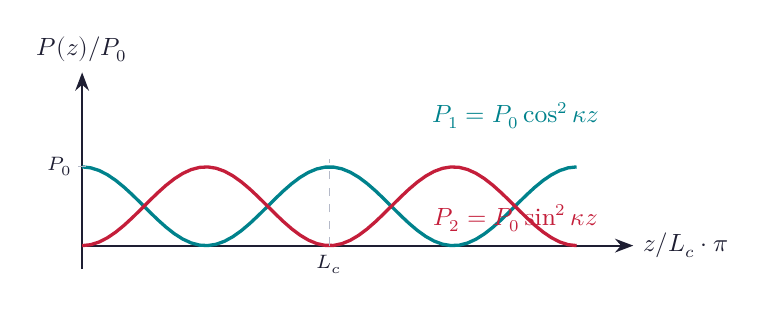
\begin{tikzpicture}[scale=1.0]
  \draw[-Stealth, thick, color=mydark] (0,0) -- (7.0,0) node[right,font=\small] {$z / L_c \cdot \pi$};
  \draw[-Stealth, thick, color=mydark] (0,-0.3) -- (0,2.2) node[above,font=\small] {$P(z)/P_0$};
  % P1 = cos^2 curve
  \draw[very thick, color=myteal, domain=0:6.28, samples=60, variable=\t]
    plot ({1.0*\t}, {cos(\t r)*cos(\t r)});
  % P2 = sin^2 curve
  \draw[very thick, color=myred, domain=0:6.28, samples=60, variable=\t]
    plot ({1.0*\t}, {sin(\t r)*sin(\t r)});
  % Coupling length marker at z = pi (half-cycle, Lc)
  \draw[dashed, thin, color=mgframe] (3.14,0) -- (3.14,1.1);
  \node[font=\scriptsize, color=mydark, below] at (3.14,0) {$L_c$};
  % Labels
  \node[font=\small\color{myteal}] at (5.5, 1.65) {$P_1 = P_0\cos^2\kappa z$};
  \node[font=\small\color{myred}] at (5.5, 0.35) {$P_2 = P_0\sin^2\kappa z$};
  % Y-axis ticks
  \node[font=\scriptsize, color=mydark, left] at (0,1.0) {$P_0$};
  \draw[thin, color=mgframe] (-0.05,1.0) -- (0.05,1.0);
\end{tikzpicture}
\end{tcolorbox}

% ===============================================================================
\section{Mach-Zehnder Modulator (MZM)}
% ===============================================================================

\begin{tcolorbox}[defbox, title={\textbf{Mach-Zehnder Modulator (MZM)}}]
A \textbf{Mach-Zehnder Modulator} is an electro-optic intensity modulator based on LiNbO$_3$. Light is split into two arms of a Mach-Zehnder interferometer; an applied electric field via the Pockels effect changes the refractive index of one (or both) arms, causing a phase shift. When the two beams recombine, constructive or destructive interference produces intensity modulation.
\end{tcolorbox}

\subsection{Structure and Operation}
\begin{enumerate}[leftmargin=*, itemsep=3pt, label=\textbf{\arabic*.}]
  \item Input light is split 50:50 at a Y-junction.
  \item Electrodes on each arm apply voltage $V$ across the waveguide; the Pockels effect changes the refractive index $\Delta n \propto r_{33} E$ where $r_{33}$ is the electro-optic coefficient ($\approx 30$\,pm/V for LiNbO$_3$).
  \item A phase shift $\Delta\phi = \pi V / V_\pi$ is induced.
  \item The two arms recombine at a second Y-junction.
\end{enumerate}

\begin{tcolorbox}[formulabox, title={\textbf{MZM Transfer Function}}]
\[
P_{out}(V) = P_{in} \cos^2\!\left(\frac{\pi V}{2V_\pi}\right) = \frac{P_{in}}{2}\left[1 + \cos\!\left(\frac{\pi V}{V_\pi}\right)\right]
\]
\textbf{Half-wave voltage $V_\pi$:} The voltage required to shift the phase by $\pi$ (switches from max to min transmission).
\[
\text{Extinction ratio (ER):} \quad r_{ext} = P_{max}/P_{min} \quad (\text{dB}) = 10\log_{10}(r_{ext})
\]
Ideal MZM: $r_{ext} \to \infty$ (perfect extinction). Practical: 20--30\,dB.
\end{tcolorbox}

\begin{tcolorbox}[tikzbox, title={Mach-Zehnder Modulator --- Structure and Output}]
\centering
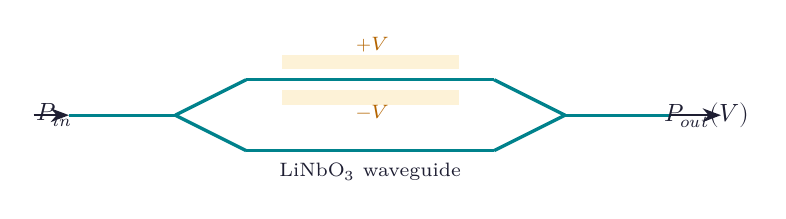
\begin{tikzpicture}[scale=0.9]
  % Splitter
  \draw[very thick, color=myteal] (0,0) -- (1.5,0);
  \draw[very thick, color=myteal] (1.5,0) -- (2.5, 0.5);
  \draw[very thick, color=myteal] (1.5,0) -- (2.5,-0.5);
  % Arms
  \draw[very thick, color=myteal] (2.5, 0.5) -- (6.0, 0.5);
  \draw[very thick, color=myteal] (2.5,-0.5) -- (6.0,-0.5);
  % Electrodes
  \fill[hdramber] (3.0, 0.65) rectangle (5.5, 0.85);
  \fill[hdramber] (3.0, 0.35) rectangle (5.5, 0.15);
  \node[font=\scriptsize\color{myamber}] at (4.25, 1.0) {$+V$};
  \node[font=\scriptsize\color{myamber}] at (4.25, 0.05) {$-V$};
  % Combiner
  \draw[very thick, color=myteal] (6.0, 0.5) -- (7.0, 0.0);
  \draw[very thick, color=myteal] (6.0,-0.5) -- (7.0, 0.0);
  \draw[very thick, color=myteal] (7.0, 0.0) -- (8.5, 0.0);
  % Labels
  \node[font=\small\color{mydark}] at (-0.2, 0) {$P_{in}$};
  \node[font=\small\color{mydark}] at (9.0, 0) {$P_{out}(V)$};
  \draw[arrow] (-0.5,0) -- (0,0);
  \draw[arrow] (8.5,0) -- (9.2,0);
  \node[font=\scriptsize\color{mydark}] at (4.25,-0.8) {LiNbO$_3$ waveguide};
\end{tikzpicture}
\end{tcolorbox}

% ===============================================================================
\section{EDFA --- Erbium-Doped Fiber Amplifier}
% ===============================================================================

\begin{tcolorbox}[defbox, title={\textbf{EDFA}}]
An \textbf{Erbium-Doped Fiber Amplifier (EDFA)} is an optical amplifier that amplifies light directly in the optical domain by stimulated emission from excited Er$^{3+}$ ions. It operates in the 1530--1565\,nm C-band (or 1570--1610\,nm L-band), exactly matching the lowest-loss window of silica fiber.
\end{tcolorbox}

\subsection{Structure and Pumping}
An EDFA consists of a few meters of silica fiber doped with Er$^{3+}$ ions. A pump laser excites the erbium ions to higher energy levels. Two standard pump wavelengths:
\begin{itemize}[leftmargin=*, itemsep=2pt]
  \item \textbf{980\,nm pump:} Three-level pumping; low noise figure ($\sim$3--4\,dB); requires WDM coupler.
  \item \textbf{1480\,nm pump:} Two-level pumping (directly pumps to metastable $^4I_{13/2}$ level); higher output power; noise figure $\sim$4--5\,dB.
\end{itemize}

\subsection{Gain Spectrum and ASE Noise}
EDFA provides gain over $\sim$35\,nm bandwidth (1530--1565\,nm). The gain spectrum is not flat; tilt compensation requires gain flattening filters (GFF).

\textbf{Amplified Spontaneous Emission (ASE):} Not all spontaneous photons escape the fiber; a fraction is guided along the fiber and amplified, producing broadband noise. The ASE power spectral density in each polarization is:
\[
S_{ASE}(\nu) = n_{sp} h\nu (G-1)
\]
where $n_{sp} \geq 1$ is the spontaneous emission factor ($n_{sp} = N_2/(N_2 - N_1)$ for a two-level system).

\textbf{Noise Figure (NF)} of an EDFA:
\[
\text{NF} = 2n_{sp}\frac{G-1}{G} + \frac{1}{G} \approx 2n_{sp} \quad \text{for large } G
\]
Minimum theoretical NF = 3\,dB (for $n_{sp} = 1$, ideal inversion).

\begin{tcolorbox}[tikzbox, title={EDFA Structure --- Forward Pumped Configuration}]
\centering
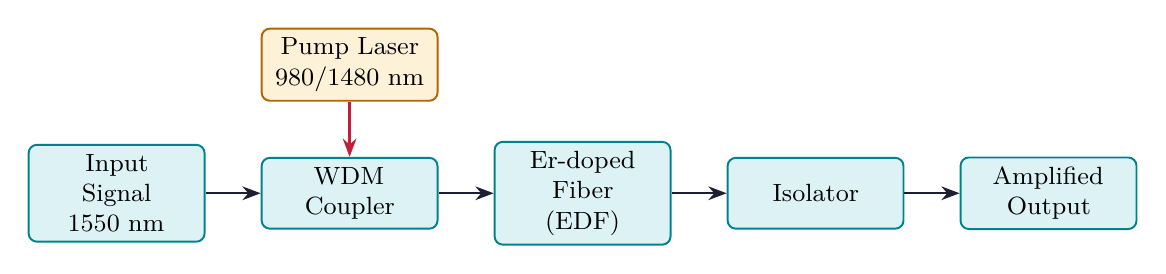
\begin{tikzpicture}[node distance=0.3cm and 0.5cm,
  sblock/.style={rectangle, draw=myteal, fill=hdrteal, text width=2.0cm,
    align=center, minimum height=0.9cm, font=\small, rounded corners=3pt, line width=0.7pt},
  pblock/.style={rectangle, draw=myamber, fill=hdramber, text width=2.0cm,
    align=center, minimum height=0.9cm, font=\small, rounded corners=3pt, line width=0.7pt}]
  \node[sblock] (in) {Input\\Signal\\1550 nm};
  \node[sblock, right=0.7cm of in] (wdm) {WDM\\Coupler};
  \node[sblock, right=0.7cm of wdm] (edf) {Er-doped\\Fiber\\(EDF)};
  \node[sblock, right=0.7cm of edf] (iso) {Isolator};
  \node[sblock, right=0.7cm of iso] (out) {Amplified\\Output};
  \node[pblock, above=0.7cm of wdm] (pump) {Pump Laser\\980/1480 nm};
  \draw[arrow] (in) -- (wdm);
  \draw[arrow] (wdm) -- (edf);
  \draw[arrow] (edf) -- (iso);
  \draw[arrow] (iso) -- (out);
  \draw[redarrow] (pump) -- (wdm);
\end{tikzpicture}
\end{tcolorbox}

% ===============================================================================
\section{Raman Amplifier}
% ===============================================================================

\begin{tcolorbox}[defbox, title={\textbf{Raman Amplifier}}]
A \textbf{Raman amplifier} exploits \textbf{Stimulated Raman Scattering (SRS)} in silica fiber to amplify an optical signal. A high-power pump transfers energy to a signal that is Stokes-shifted by $\sim$13\,THz (corresponding to $\sim$100\,nm red shift). The transmission fiber itself acts as the gain medium.
\end{tcolorbox}

\subsection{Stimulated Raman Scattering (SRS)}
A pump photon at frequency $\nu_p$ interacts with a silica molecular vibration to produce a signal photon at lower frequency $\nu_s = \nu_p - \nu_v$ (Stokes shift) and a phonon. The Raman gain coefficient $g_R \approx 6\times10^{-14}$\,m/W at $\lambda_p = 1450$\,nm.

\begin{tcolorbox}[formulabox, title={\textbf{Raman Gain}}]
\[
G_R = \exp\!\left(\frac{g_R P_p L_{eff}}{A_{eff}}\right)
\]
where $P_p$ is pump power, $L_{eff} = [1 - e^{-\alpha_p L}]/\alpha_p$ is the effective length, $A_{eff}$ is effective mode area.
\end{tcolorbox}

\subsection{Distributed vs Lumped Raman Amplification}
\begin{itemize}[leftmargin=*, itemsep=3pt]
  \item \textbf{Distributed Raman:} The transmission fiber is used as the gain medium with backward pumping. The signal is amplified continuously along the fiber, reducing the noise figure dramatically. Best OSNR performance.
  \item \textbf{Lumped (discrete) Raman:} A separate short high-nonlinearity fiber (HNF) provides concentrated gain. Simpler pump management.
\end{itemize}

\subsection{EDFA vs Raman Amplifier Comparison}
\par\noindent
{\renewcommand{\arraystretch}{1.55}
\begin{tabularx}{\linewidth}{|B{3.5cm}|Y|Y|}
\hline
\textbf{Parameter} & \textbf{EDFA} & \textbf{Raman Amplifier} \\
\hline
Gain medium & Er-doped fiber & Transmission fiber (silica) \\
\hline
Gain band & 1530--1565\,nm (C-band) & Flexible ($\sim$100\,nm from pump) \\
\hline
Pump wavelength & 980/1480\,nm & $\sim$100\,nm below signal \\
\hline
Gain flatness & Requires GFF & Inherently broad but uneven \\
\hline
Noise figure & $\sim$3--6\,dB & $<$0\,dB (effective; distributed) \\
\hline
Amplification type & Lumped & Distributed or lumped \\
\hline
Cost/complexity & Moderate & Higher pump power needed \\
\hline
\end{tabularx}}

% ===============================================================================
% QUICK REVISION PAGE
% ===============================================================================
\newpage
\begin{center}
  {\large\bfseries\color{myred} Quick Revision --- Module 4}\\[3pt]
  {\small\color{mydark} Optical Switches, Couplers, and Amplifiers $|$ PE-EC801B}
\end{center}
\noindent{\color{myred}\rule{\linewidth}{1.2pt}}
\vspace{4pt}

\begin{tcolorbox}[formulabox, title={\textbf{Key Formulas at a Glance}}]
\renewcommand{\arraystretch}{1.35}
\begin{tabularx}{\linewidth}{B{5.0cm} X}
Coupler power transfer & $P_1 = P_0\cos^2(\kappa L)$; \quad $P_2 = P_0\sin^2(\kappa L)$ \\[4pt]
Coupling length & $L_c = \pi/(2\kappa)$ (full transfer) \\[4pt]
MZM transfer function & $P_{out} = P_{in}\cos^2(\pi V/2V_\pi)$ \\[4pt]
EDFA ASE noise PSD & $S_{ASE} = n_{sp} h\nu(G-1)$ \\[4pt]
EDFA noise figure & $\text{NF} \approx 2n_{sp}$ (large $G$); min $= 3$\,dB \\[4pt]
Raman gain & $G_R = \exp(g_R P_p L_{eff}/A_{eff})$ \\[4pt]
Raman Stokes shift & $\Delta\nu \approx 13$\,THz; \quad $\Delta\lambda \approx 100$\,nm at 1550\,nm \\[4pt]
\end{tabularx}
\end{tcolorbox}

\begin{tcolorbox}[defbox, title={\textbf{One-Line Definitions}}]
\begin{itemize}[leftmargin=*, itemsep=2pt, topsep=0pt]
  \item \textbf{Directional coupler:} 4-port device transferring power via evanescent field overlap between two waveguides.
  \item \textbf{Coupling coefficient $\kappa$:} Rate of power transfer per unit length in a directional coupler.
  \item \textbf{MZM:} Mach-Zehnder Modulator; electro-optic intensity modulator using LiNbO$_3$ Pockels effect.
  \item \textbf{$V_\pi$:} Voltage causing $\pi$ phase shift in MZM; half-wave voltage.
  \item \textbf{EDFA:} Er-doped fiber amplifier; all-optical gain in 1530--1565\,nm C-band.
  \item \textbf{ASE:} Amplified Spontaneous Emission; broadband noise generated in optical amplifiers.
  \item \textbf{SRS:} Stimulated Raman Scattering; pump photon excites molecular vibration, emits Stokes-shifted signal photon.
  \item \textbf{Distributed Raman:} Uses the transmission fiber as gain medium; best noise performance.
  \item \textbf{Noise figure (NF):} Degradation of OSNR through an amplifier; minimum theoretical = 3\,dB.
\end{itemize}
\end{tcolorbox}

\begin{tcolorbox}[exambox, title={\textbf{Frequently Asked / Viva Questions}}]
\begin{enumerate}[topsep=0pt, label=\textbf{Q\arabic*.}, itemsep=5pt]
  \item \Q{What is the principle of operation of a directional coupler?}
    When two waveguides are placed sufficiently close, their evanescent fields overlap. The resulting coupled mode equations show that power oscillates sinusoidally between the two guides with period $L_c = \pi/(2\kappa)$.
  \item \Q{What is the coupling length and how is it related to $\kappa$?}
    $L_c = \pi/(2\kappa)$ is the length at which all power transfers from guide 1 to guide 2. $\kappa$ (m$^{-1}$) depends on the overlap integral of the evanescent fields.
  \item \Q{What is the half-wave voltage $V_\pi$ of an MZM?}
    $V_\pi$ is the voltage needed to cause a phase shift of exactly $\pi$ in one arm of the MZM, switching the output from maximum to minimum (or vice versa). Lower $V_\pi$ means less drive power needed.
  \item \Q{Why is LiNbO$_3$ used in MZMs?}
    LiNbO$_3$ has a large electro-optic (Pockels) coefficient $r_{33} \approx 30$\,pm/V, enabling efficient phase shifting with moderate voltage. It also has low optical loss in the 1310--1550\,nm bands.
  \item \Q{What are the two pump wavelengths for EDFA and their trade-offs?}
    980\,nm: lower noise figure ($\sim$3--4\,dB), three-level pumping, lower output power. 1480\,nm: higher saturation power, two-level pumping, slightly higher NF ($\sim$4--5\,dB). 980\,nm preferred for low-noise preamplification.
  \item \Q{What is ASE in EDFA? How does it affect system performance?}
    ASE is spontaneous emission from excited Er$^{3+}$ ions that is guided and amplified. It degrades OSNR (optical signal-to-noise ratio) and limits the number of amplifier cascades in a chain.
  \item \Q{What is the minimum theoretical noise figure of an EDFA?}
    3\,dB. This corresponds to $n_{sp} = 1$ (complete population inversion) and large gain $G \gg 1$.
  \item \Q{Explain stimulated Raman scattering in the context of fiber amplification.}
    A high-power pump photon ($\nu_p$) interacts with a silica phonon, losing energy to produce a Stokes signal photon at $\nu_s = \nu_p - \nu_{phonon}$. If a signal is present at $\nu_s$, it triggers more SRS events --- stimulated Raman amplification.
  \item \Q{What are the advantages of distributed Raman amplification?}
    The gain is spread over the entire span, keeping the signal power higher throughout the fiber. This reduces the effective noise figure and improves OSNR compared to lumped amplification. No discrete amplifier components needed in the span.
  \item \Q{Classify optical switches and state their switching speeds.}
    Mechanical: ms--s; Electro-optic: ps--ns; Acousto-optic: $\mu$s; Thermo-optic: ms; MEMS: ms.
  \item \Q{What is the extinction ratio of an MZM?}
    $\text{ER} = P_{max}/P_{min}$. An ideal MZM has infinite ER (perfect extinction). Practical devices achieve 20--30\,dB due to waveguide asymmetries and electrode misalignment.
\end{enumerate}
\end{tcolorbox}

\begin{tcolorbox}[tikzbox, title={EDFA vs Raman --- Quick Comparison}]
\centering
{\renewcommand{\arraystretch}{1.45}
\begin{tabularx}{\linewidth}{|B{3.2cm}|Y|Y|}
\hline
\textbf{Feature} & \textbf{EDFA} & \textbf{Raman} \\
\hline
Gain band & 1530--1565\,nm & Tunable with pump \\
\hline
Noise figure & $\geq$3\,dB & $<$0\,dB effective (dist.) \\
\hline
Amplifier type & Lumped & Distributed or lumped \\
\hline
Gain medium & Er-doped fiber & Transmission fiber \\
\hline
Pump $\lambda$ & 980/1480\,nm & $\sim$1450\,nm (for 1550) \\
\hline
\end{tabularx}}
\end{tcolorbox}

\end{document}
